\section{Objective 4: Synchronise Logging of Flight Telemetry and Radar Measurements}

\subsection{Introduction}

To synchronise flight telemetry and radar measurements, a pilot-initiated control signal must be interpreted, processed, and transmitted through the system. The signal travels from the pilot transmitter to the receiver, then to the flight controller, and finally to the \gls{sbc}, which triggers \gls{sdr} logging. This signal path is shown in Figure~\ref{fig:activation-signal-flow}.

\begin{figure}[!htbp]
    \centering
    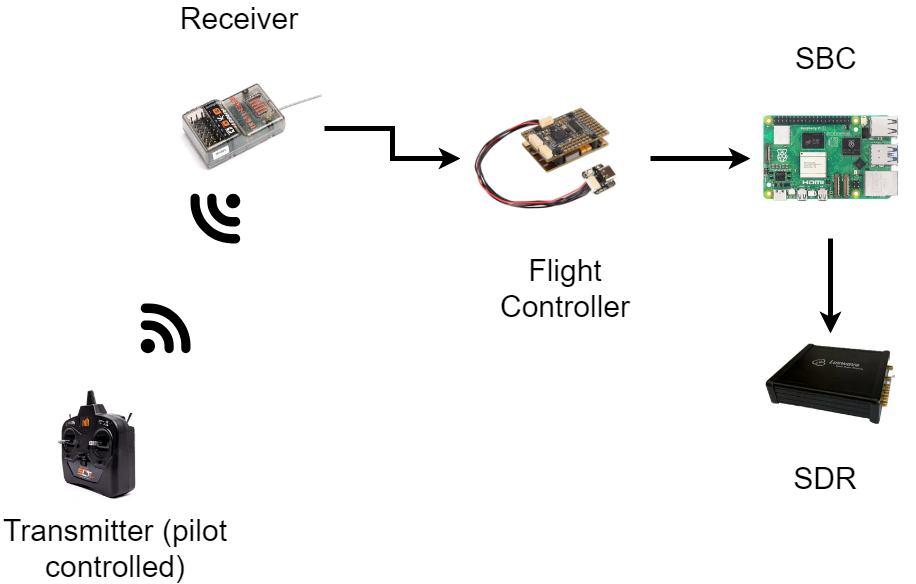
\includegraphics[width=0.5\textwidth]{ch4-4_images/Activation signal diagram.drawio.png}
    \caption{Activation signal flow starting at the pilot transmitter and ending at the \gls{sdr}.}
    \label{fig:activation-signal-flow}
\end{figure}

Progress toward this objective has included researching and procuring a suitable \gls{sbc}, completing its initial setup, and conducting a communication trial between the \gls{sbc} and a simulated flight-controller signal.

\subsection{Methodology}


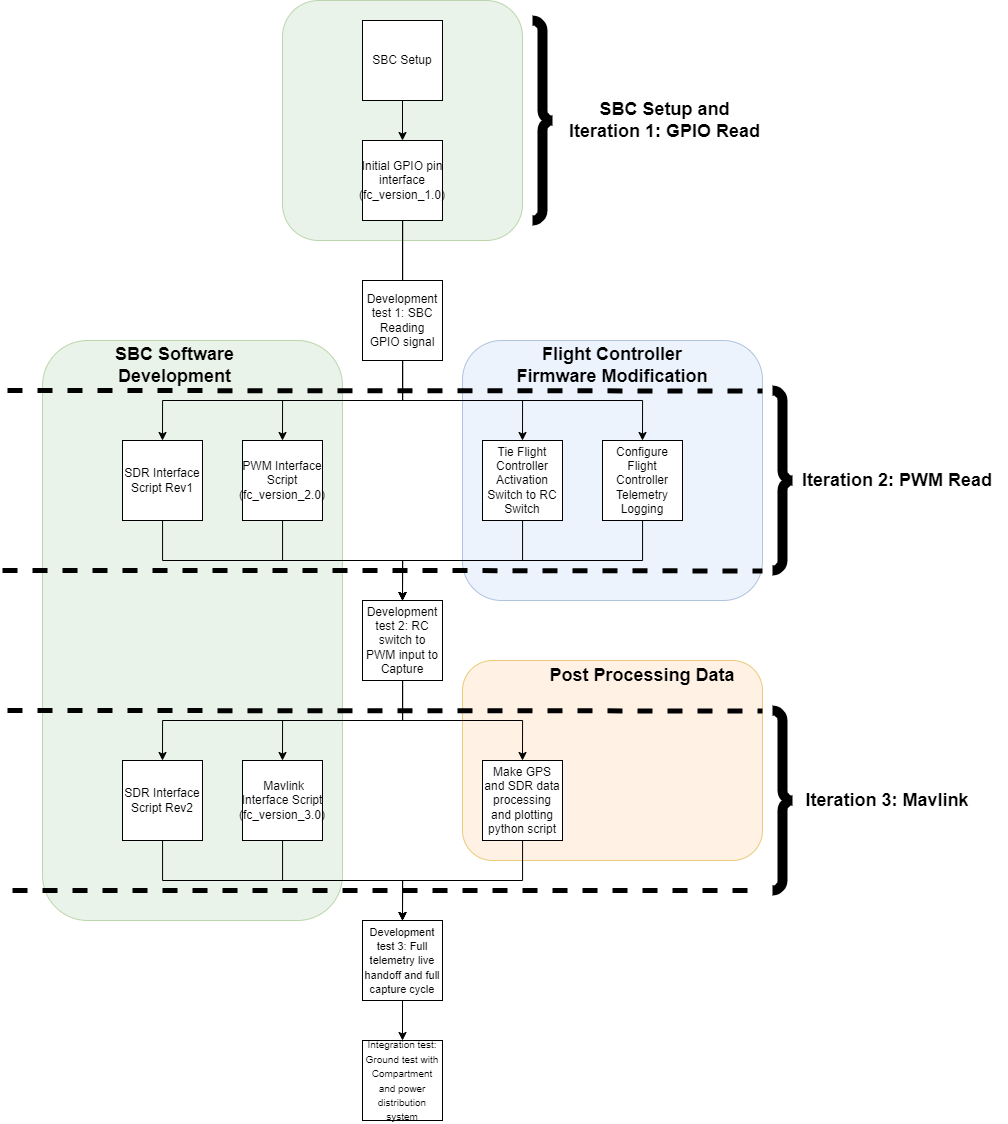
\includegraphics[width=0.8\textwidth]{ch4-4_images/Control System Development Cycle.drawio.png}



\subsubsection{SBC Setup and Iteration 1: GPIO Read}

\textit{SBC Setup} 

First, requirements of the \gls{sbc} were identified. The hardware requirements for the \gls{sbc} were derived from the \gls{sdr} datasheet, which specifies the need for a high-speed USB 2.0 interface (480 Mb/s)~\cite{luswavePUPDUAL24C}. Additionally, the \gls{sbc} should provide sufficient processing capability to support potential future expansion of onboard processing capability, placing requirements on CPU performance and RAM capacity.

Consequently, a Raspberry Pi 5 with 16 GB of RAM was selected and procured. In addition to satisfying the hardware requirements, Raspberry Pi devices were selected because of their well-supported software ecosystem and prior use in drone-mounted radar research applications~\cite{kawkaSwarmDronesDetection2025,lopezUnmannedAerialVehicleBased2022,coulibalyBlockchainSoftwareDefinedRadio2025,aliDesignImplementationFMCW2017}. A protective case and active cooler were also acquired to secure the device on board the drone and manage \gls{cpu} temperature during \gls{sdr} operation.

The Raspberry Pi 5 was physically assembled and configured with a lightweight Ubuntu 22.04 operating system. The installation process used an imager to write the Ubuntu disk image to a 64 GB microSD card. The card was then inserted into the Raspberry Pi 5, and the system was booted to verify the operating-system installation.

A remote development workflow was then configured to develop and test the Python script used to read the \gls{gpio} pin. Native development on the Raspberry Pi was avoided due to its lower performance compared with a desktop computer. Instead, \gls{ssh} was configured and integrated with an \gls{ide} to enable remote development.

\gls{ssh} provides a secure remote connection between a host and a remote computer. In this setup, the desktop computer was used as the development machine, and the Raspberry Pi 5 was used as the remote host. The setup commands are shown in Listing~\ref{lst:ssh-setup}. These commands install the \gls{ssh} server, enable the \gls{ssh} service at boot, and allow incoming \gls{ssh} connections through the firewall. The successful \gls{ssh} connection is shown in \hyperlink{appendix:ssh-connection}{Appendix X}.

\begin{lstlisting}[language=bash,caption={The commands used to setup SSH connection between the Raspberry Pi and a remote computer.},label={lst:ssh-setup}]
sudo apt install openssh-server
sudo systemctl enable ssh
sudo ufw allow ssh
\end{lstlisting}

The \gls{ssh} connection was then integrated with VS Code using the Microsoft \textit{Remote - \gls{ssh}} extension. The \gls{ssh} configuration file on the development laptop was updated with the Raspberry Pi's IP address and username, after which VS Code was connected to the Raspberry Pi through the remote \gls{ssh} interface.

\textit{Iteration 1: GPIO Read}

To allow the Raspberry Pi to read \gls{gpio} pins, the required \gls{gpio} packages were installed. The installation command is shown in Listing~\ref{lst:gpio-package-install}. The package \texttt{python3-lgpio} provides Python bindings and low-level \gls{gpio} access, and \texttt{gpiod} provides terminal tools for inspecting and manipulating \gls{gpio} pins.

\begin{lstlisting}[language=Bash,caption={Bash command used to install python \gls{gpio} library.},label={lst:gpio-package-install}]
sudo apt install python3-lgpio gpiod
\end{lstlisting}

The \texttt{lgpio} package is used interface with \gls{gpio} pins on a level too low in abstraction for the application. The package to use for interfacing with the pins at a higher abstraction level was called \texttt{rpi-lgpio}, which uses \texttt{lgpio} as a backened. The package can only be installed with \texttt{pip}, so a Python virtual environment was created. The virtual environment setup and installation of \texttt{rpi-lgpio} is shown in Listing~\ref{lst:rpi-lgpio-install}

\begin{lstlisting}[language=Bash, caption=commands used to create the python virtual environment and install \texttt{rpi-lgpio},label={lst:rpi-lgpio-install}]
wget http://abyz.me.uk/lg/lg.zip
unzip lg.zip
cd lg
make
sudo make install
python3 -m venv gpio-env
source gpio-env/bin/activate
pip install rpi-lgpio

\end{lstlisting}

After installing the packages, a Python script was created to read a \gls{gpio} pin and respond when an external component pulls the signal high. The script is shown in Listing~\ref{lst:gpio-script}.

\begin{lstlisting}[language=python,caption={Python script used to run on the Raspberry Pi to monitor one of the \gls{gpio} pins.},label={lst:gpio-script}]
#!/usr/bin/env python3
import RPi.GPIO as GPIO # Uses rpi-lgpio backend automatically
from time import sleep
import signal

# Setup
GPIO_PIN = 17
GPIO.setmode(GPIO.BCM)
GPIO.setup(GPIO_PIN, GPIO.IN, pull_up_down=GPIO.PUD_DOWN)

print("Sensing 3.3V High...")

try:
    while True:
        if GPIO.input(GPIO_PIN):
            print("Pin High")
            sleep(1)
except KeyboardInterrupt:
    print("Stopping...")
finally:
    GPIO.cleanup()
pause()
\end{lstlisting}

To verify the program, an Arduino Uno R3 was used to generate an input signal for a \gls{gpio} pin. Because the Raspberry Pi 5 uses 3.3 V logic and the Arduino Uno R3 outputs 5 V logic, a resistor divider was used to reduce the signal to approximately 3.3 V and protect the Raspberry Pi.

This process concluded the development of the first software that was made for the flight controller. 



\subsubsection{Iteration 2: PWM Read}

After the first software iteration was tested and confirmed working as expected, a new iteration was created. This iteration now reads in the specific signal sent from the flight controller output to the GPIO pins, which is \gls{pwm}. This iteration was split into several parallel tasks. On the flight controller side, outputting a specific PWM channel from an activation switch on the transmitter was a task, as was configuring the flight controller for telemetry logging. On the \gls{sbc} side, a refined script to interface with the flight controllers signals was made, and setting up the \gls{sbc} to interface with the Radar (including the function to run the SDR capture and setting up the software requirements to run the SDR) was it's own task. These four tasks are outlined in this section.



\textit{Tie Flight Controller Activation Switch to RC Switch}

Before doing anything, the flight controller had to be conencted to a Desktop PC to be able to interface with the device properly. This was done by installing and using Mission Planner.

Upon configuring, the task then became to tie a PWM output channel to an RC switch on the transmitter. THis PWM output channel would then be read by the SBC, which would activate/deactivate the radar capture accordingly. 

On the transmitter in possession, there were 8 physical switches. The switch that was deemed suitable was tied to RC channel 15 using the transmitter settings.

In Mission Planner, RC Channel 15 was then tied to servo output 8. After configuring, the output signal was scoped with an oscilloscope and confirmed working as intended. 

This development concluded with a successful tying of the transmitter physical switch to a servo output channel on the flight controller, enabling the transmitter to have a physical switch dedicated to radar capture.
What to bring up:
\begin{enumerate}
    \item Signal flow point that we are at
    \item What PWM is
    \item Tying the PWM channel on the drone and outputting from the flight controller
\end{enumerate}

\textit{Configure Flight Controller Telemetry Logging}

It was also imperative to gain an understanding of how the flight controller recorded telemetry and configure the logging in such a way to suit the application. That was the objective of this section. 

It was found that when the host PC connects to the flihgt controller, the flight controller makes a .tlog file and continues to write to the .tlog file until the connection is terminated.

The telemetry log only records \gls{gps} when the drone is armed. This setting did not suit the project, as the drone needed to be disarmed for the majority of the project. To enable \gls{gps} logging while disarmed, a parameter was changed in the config file in Mission Planner. 

\begin{enumerate}
    \item How the flight controller logs telemetry
    \item Setting when to record telemetry
    \item getting the telemetry logs off from the flight controller
\end{enumerate}


\textit{PWM Interface Script}

At this stage of development, the flight controller interfaces with the \gls{sbc} via \gls{pwm}. Whether a signal is logic HIGH or logic LOW is determined by the pulse width of the transmission. For the flight controller signal, a pulse width below 1300 $\mu s$ is logic LOW, and a pulse width above 1700 $\mu s$ is logic HIGH. This is the logic embedded into the script that the \gls{sbc} uses to interface with the flight controller. 

The input logic is controlled by the \texttt{RCInput} class, which is shown in Listing~\ref{lst:RCInput-class}

\begin{lstlisting}[language=Python, caption=RCInput class used to control PWM input logic, label={lst:RCInput-class}]
import RPi.GPIO as GPIO
import time

from .config import RC7_PIN, RC8_PIN
from .config import PWM_HIGH, PWM_LOW


class RCInput:

    def __init__(self):

        self.rc7_pulse_width = 0
        self.rc8_pulse_width = 0

        self.rc7_high = False
        self.rc8_high = False

        self.rc7_rising_time = None
        self.rc8_rising_time = None

        self.rc7_last_low = 0
        self.rc8_last_low = 0

        GPIO.setup(RC7_PIN, GPIO.IN, pull_up_down=GPIO.PUD_DOWN)

        GPIO.setup(RC8_PIN, GPIO.IN, pull_up_down=GPIO.PUD_DOWN)

        GPIO.add_event_detect(RC7_PIN, GPIO.BOTH, callback=self.rc7_callback)

        GPIO.add_event_detect(RC8_PIN, GPIO.BOTH, callback=self.rc8_callback)

    def rc7_callback(self, channel):

        if GPIO.input(channel):

            # Rising edge
            self.rc7_rising_time = time.monotonic_ns()

        else:

            # Falling edge
            if self.rc7_rising_time is not None:

                falling_time = time.monotonic_ns()

                self.rc7_pulse_width = (falling_time - self.rc7_rising_time) / 1000

                self.rc7_rising_time = None

                if self.rc7_pulse_width > PWM_HIGH:

                    self.rc7_high = True

                elif self.rc7_pulse_width < PWM_LOW:

                    self.rc7_high = False

    def rc8_callback(self, channel):

        if GPIO.input(channel):

            # Rising edge
            self.rc8_rising_time = time.monotonic_ns()

        else:

            # Falling edge
            if self.rc8_rising_time is not None:

                falling_time = time.monotonic_ns()

                self.rc8_pulse_width = (falling_time - self.rc8_rising_time) / 1000

                self.rc8_rising_time = None

                if self.rc8_pulse_width > PWM_HIGH:

                    self.rc8_high = True

                elif self.rc8_pulse_width < PWM_LOW:

                    self.rc8_high = False
\end{lstlisting}

The main flow of the program is controlled by the main.py script, which is shown in Listing \ref{lst:pwm_interface_main}. The script initialises the Raspberry Pi GPIO interface and creates instances of the RC input, radar, GPS, and display classes. It then continuously monitors the RC channels, starting a radar capture when the appropriate input transitions high and activating GPS when the corresponding input is high. Runtime and capture information are written to output.txt, while the display is periodically updated with the current system state. When the program is interrupted or terminated, it performs a shutdown routine that cleans up the environment. 

\begin{lstlisting}[language=Python, caption=Main file of \gls{pwm} interface script, label={lst:pwm_interface_main}]
#!/usr/bin/env python3

import RPi.GPIO as GPIO
import time
import signal

from files.rc_input import RCInput
from files.radar import Radar
from files.gps import GPS
from files.display import display
from files.config import DISPLAY_REFRESH

# ============================================================
# GLOBAL STATE
# ============================================================

start_time = time.monotonic()

# ============================================================
# INITIALISE
# ============================================================

GPIO.setmode(GPIO.BCM)

rc = RCInput()

radar = Radar()

gps = GPS()

# ============================================================
# OUTPUT
# ============================================================


def update_output(gps, radar):
    with open("output.txt", "w") as file:
        file.write(f"GPS Activation time: {gps.activation_time}\n")
        file.write(f"Radar capture times: {radar.capture_times}\n")


# ============================================================
# MAIN LOOP
# ============================================================


def main():

    global drone_armed
    global start_time

    print("Starting drone radar interface...")
    open("output.txt", "w")  # overwrite previous file

    try:

        while True:

            runtime = time.monotonic() - start_time

            # ------------------------------------------------
            # Radar Capture
            # ------------------------------------------------

            if rc.rc7_high and rc.rc7_last_low:

                radar.start_capture(runtime)
                update_output(gps, radar)
                radar.stop_capture()
                rc.rc7_last_low = 0

            if not rc.rc7_high:
                rc.rc7_last_low = 1

            # ------------------------------------------------
            # GPS
            # ------------------------------------------------

            if rc.rc8_high:

                gps.activate()
                update_output(gps, radar)

            # ------------------------------------------------
            # DISPLAY
            # ------------------------------------------------

            display(rc, radar, gps, runtime)

            time.sleep(DISPLAY_REFRESH)

    except KeyboardInterrupt:

        shutdown()


# ============================================================
# SHUTDOWN
# ============================================================


def shutdown():

    print("\nCleaning up...")

    GPIO.cleanup()


def signal_handler(signal_number, frame):

    shutdown()

    exit(0)


signal.signal(signal.SIGINT, signal_handler)

signal.signal(signal.SIGTERM, signal_handler)


# ============================================================
# START
# ============================================================

if __name__ == "__main__":

    main()
\end{lstlisting}


\begin{enumerate}
    \item The PWM interface
    \item Overview of the classes 
    \item Main function flow
\end{enumerate}

\textit{SDR Interface function Rev1}

The PWM interface script was modified to enable the use of Bash commands to activate the script that initiates radar capture. Following this, the class to handle the radar capture script was implemented. This function is shown in Listing \ref{lst:radarclass_pwm}. The Radar class manages the state of radar captures and records basic capture information. When a capture is started, it prevents duplicate captures, increments the capture count, records the capture time, and adds it to a list of previous capture times. The \texttt{stop\_capture()} method ends the active capture, while the commented \texttt{subprocess.run()} shows where the external radar acquisition command can be executed.

\begin{lstlisting}[language=Python, caption=Radar capture class implemented in pwm interface script, label={lst:radarclass_pwm}]
import time
import subprocess


class Radar:

    def __init__(self):

        self.capturing = False
        self.capture_count = 0
        self.last_capture_time = None

        self.capture_times = []

    def start_capture(self, runtime):

        if self.capturing:
            return

        self.capturing = True

        self.capture_count += 1

        self.last_capture_time = runtime

        self.capture_times.append(self.last_capture_time)

        print("Radar capture started")

        # Start radar here
        # subprocess.run(
        #     """
        #     sudo ./build-arm64/pupradar_capture --firmware firmware/SDR_USB_FW.hex --duration 5 --fc-low 24.00e9 --fc-high 26e9 --sweep-time 1 --samp-num 4 --out ~/SDR-data/0209_pi/0209_2GHz_128_0-5ms_loopback_rx1_01 --rx 1
        #     """,
        #     shell=True,
        #     executable="/bin/bash",
        #     check=True,
        # )

    def stop_capture(self):

        if not self.capturing:
            return

        self.capturing = False

        print("Radar capture stopped")
\end{lstlisting}



\begin{enumerate}
    \item Getting Python to run shell code
    \item Setting the sticky capture function
    \item The execution capture cycle
\end{enumerate}





\subsubsection{Iteration 3: Mavlink}

Likewise from the second iteration, a single python 3 program on 
the \gls{sbc} handled both the flight controller and 
the \gls{sdr} in one loop. 

Again, the code was split by device, a \texttt{Drone} class, which
handled the flight controller interface, a \texttt{Radar} class, which
handled the radar interface, and a small \texttt{main.py} script to
run the overall program. 

The benefit to the program being one one system was the fact that
all the timing was able to use a single clock, which was \texttt{runtime} (seconds
elapsed since the start of the program). Both the telemetry
log and the radar used this value, and shared the same time base 
which is what made synchronisation possible. 


\textit{Mavlink Interface}

The \gls{sbc} interfaced with the drone via Mavlink, a 
communication protocol used to interface between flight controllers
and desktop computers (which the Raspberry Pi 5 running Ubuntu
has a similar architecture to). The physical connection was over 
\gls{usb} serial, and the software interface was
handled by the \texttt{pymavlink} python package. 

The script blocked until it received a \texttt{HEARTBEAT} signal
which confirmed the link and gave the target system and component IDs 
to be used by later commands. Instead of relying on default stream rates, the script
sent \texttt{MAV\_CMD\_SET\_MESSAGE\_INTERVAL} commands
to request each message at a fixed rate. The message 
ID's of the key messages is shown in Table \ref{tab:mavlink_messages}.


\begin{table}[htbp]
    \centering
    \caption{MAVLink messages requested from the flight controller and their use.}
    \label{tab:mavlink_messages}
    \begin{tabular}{llcl}
        \toprule
        \textbf{Message} & \textbf{ID} & \textbf{Rate} & \textbf{Used for} \\
        \midrule
        \texttt{GPS\_RAW\_INT}         & 24  & 1\,Hz   & Fix type, satellites, latitude, longitude \\
        \texttt{GLOBAL\_POSITION\_INT} & 33  & 5\,Hz   & Altitude (AMSL and relative), groundspeed \\
        \texttt{ATTITUDE}              & 30  & 5\,Hz   & Roll, pitch, yaw \\
        \texttt{BATTERY\_STATUS}       & 147 & 1\,Hz   & Voltage, current, remaining capacity \\
        \texttt{VFR\_HUD}              & 74  & 2\,Hz   & Requested but not parsed \\
        \texttt{RC\_CHANNELS}          & 65  & 5\,Hz   & Channel 15 (radar trigger) \\
        \texttt{HEARTBEAT}             & 0   & Default & Armed state, flight mode \\
        \bottomrule
    \end{tabular}
\end{table}


on each loop in the \texttt{main.py} file, \text{update()} drained
every queued message with non blocking \texttt{recv\_match(blocking=False)},
and so the program was never stalled by a slow linkm as the stored
value was always the latest received. 

Raw Mavlink fields were converted to \gls{si} units upon reception,
including converting lattitude and longitude from degE7 to degrees, 
altitude from milimetres to metres, and voltage from millivolts to volts.

The armed status of the drone was read from the \texttt{MAV\_MODE\_FLAG\_SAFETY\_ARMED} 
bit of \texttt{HEARTBEAT.base\_mode}, and the flight mode
was decoded with \texttt{mode\_string\_v10}. The \texttt{gps\_ready} state was changed based on whether a fix to three 
or more satellites was present. 

Same from iteration 2, the radar was triggered from a switch on the pilot's 
transmitter which was mapped to channel 15. However, instead of reading in 
a PWM signal output from the flight controller, the signal was read through the \texttt{RC\_CHANNELS}
MAVlink message. 

The trigger logic remained the same; rising edge detection. A capture was 
requested by the main script to the radar only when the pulse width was above 1800 $ \mus$.
The capture logic was sticky; the switch had to be seen as low before a new 
capture could be requested (which was a pulse width below 1200 $\mu s$). The 
sticky logic prevented one switch from firing repeatedly, ignored the noise
in the invalid range, and prevented a switch left high at startup from requesting 
a capture. Both pulse width parameters can be changed easily in the config file. 
Buffering was not used; if the radar was still busy, the request was rejected 
and a message printed, instead of the request being queued. The reason for this 
was




\textit{SDR Interface}

\textit{GPS and SDR Processing and Plotting}



\subsection{Results and Discussion}

\subsubsection{Development test 1: GPIO Read}

\subsubsection{Development test 2: RC Switch to PWM Capture Cycle}

\subsubsection{Development test 3: Full telemetry live handoff and full capture cycle}

\subsubsection{Ground Test: Full Integration with other subsystems on the ground demonstrating full capture cycle and logging}

\subsection{Summary}